\section{User Level ISA Validation}
\label{sec:str7_validation_user_level}

When performing the validation of the ISA at the \textit{user level} we are only interested in the instructions that the processor can execute when running at the \textit{user mode}.
The \textit{user mode} is usually the most used mode on a processor (whenever the processor has multiple execution modes, which the ARM7TDMI has).
It is used to run the non-system dependent part of the applications.
Whenever an application needs to access the system (write on the screen, read the input from the keyboard, etc), it executes an special instruction (usually we call it \textit{system call}) which switches the processor to \textit{system mode} to perform the required operation.

The interest on performing a validation of \textit{user level} instructions resides on the difficulty to perform complete tests when using the \textit{system level} instructions (as we will see on Section~\ref{sec:str7_validation_system_level}).

\begin{figure}[!h]
	\begin{center}
		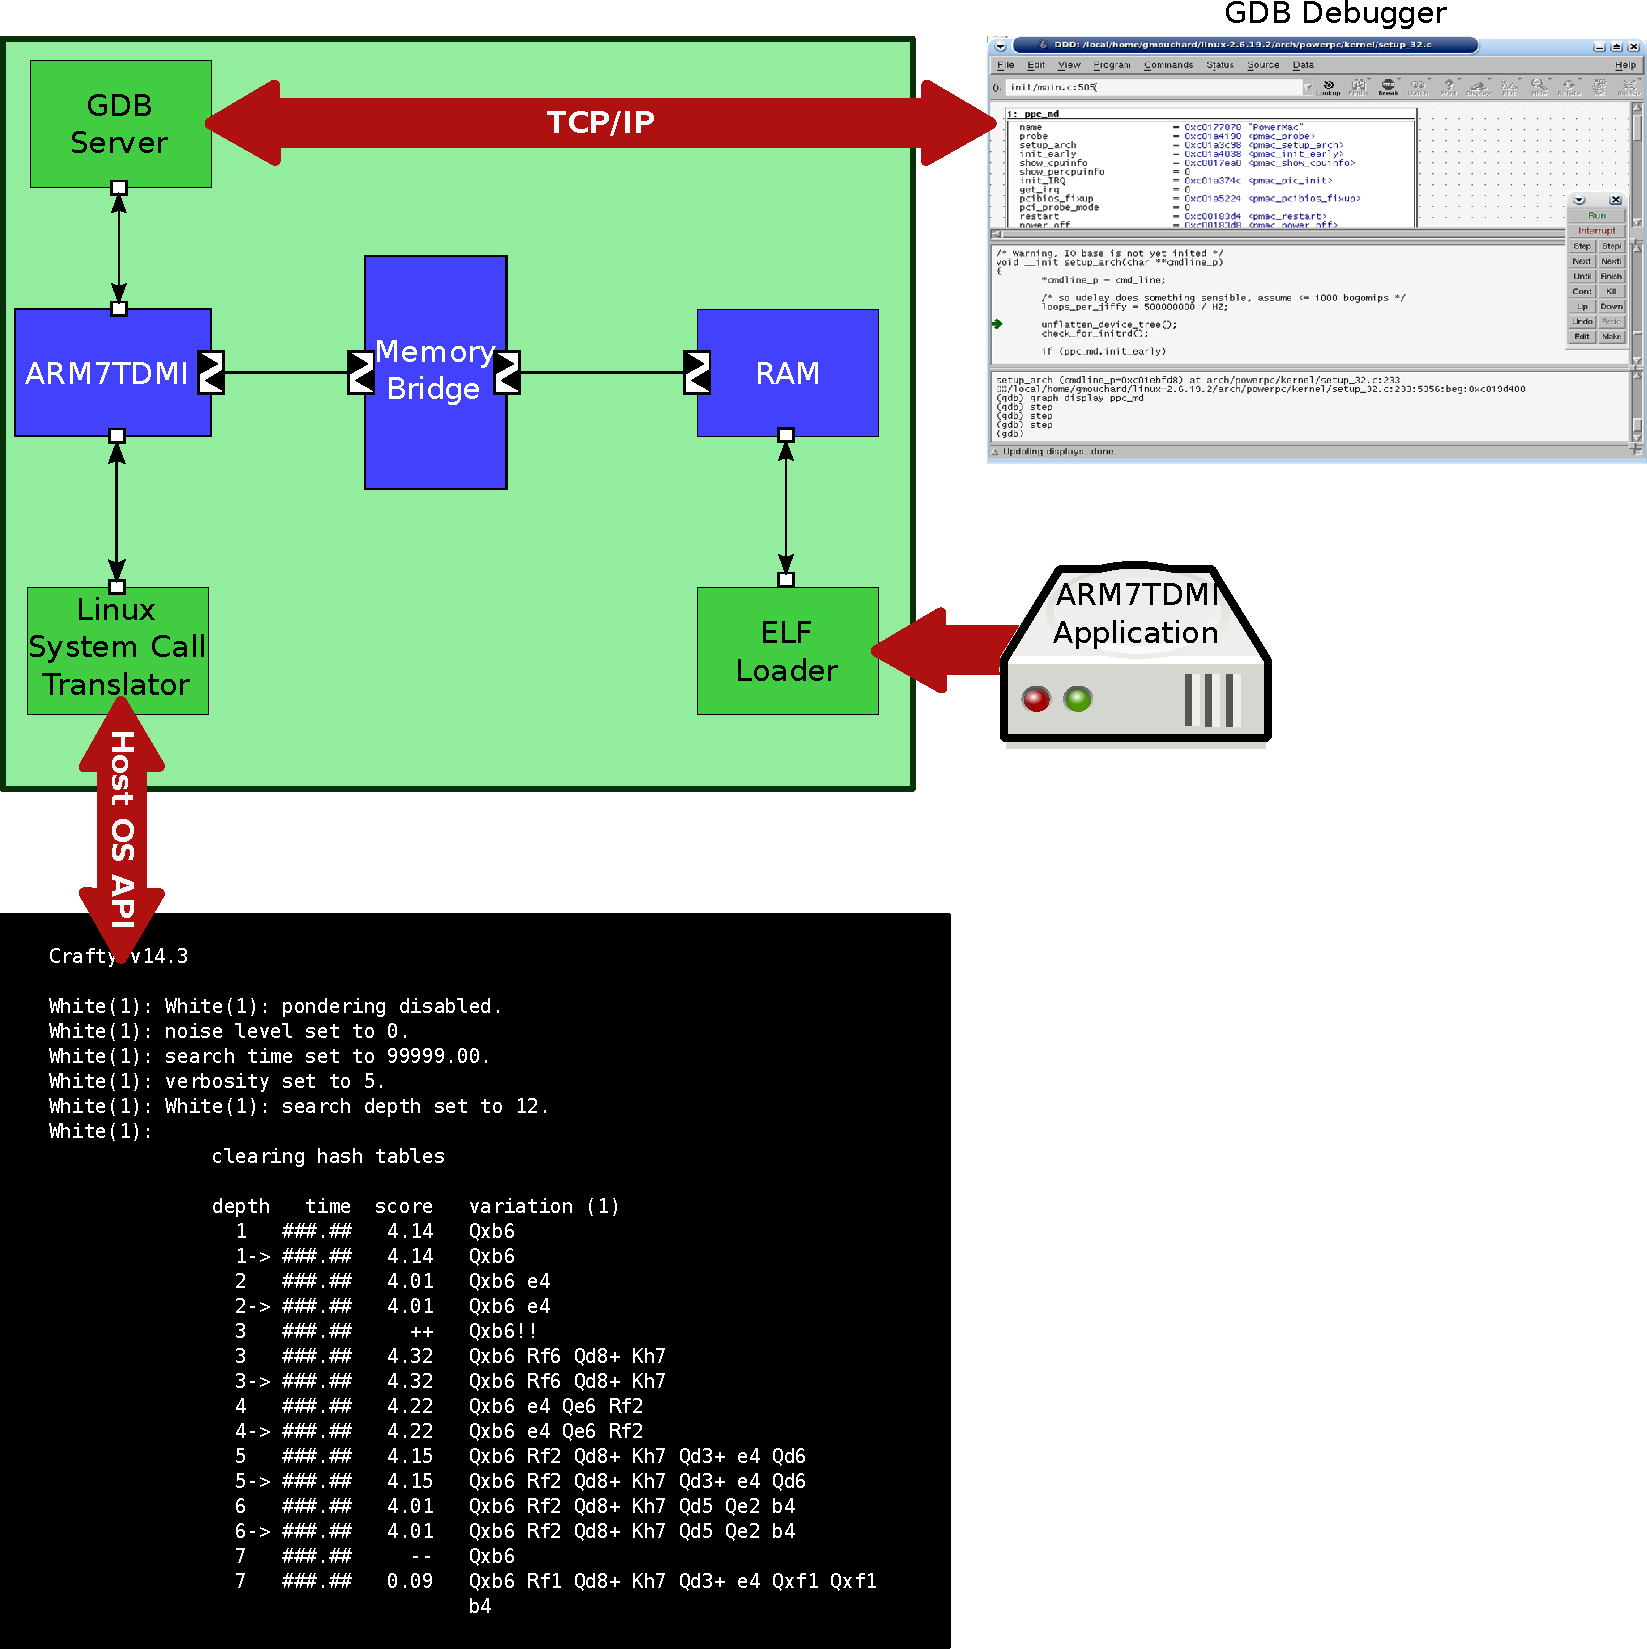
\includegraphics[width=\textwidth]{str7_validation/figures/ARM7TDMI_user_level.pdf}
	\end{center}
	\caption{ARM7TDMI schematic architecture to run applications at user level.}
	\label{fig:str7_validation_user_level}
\end{figure}

In order to validate only the \textit{user level} ISA, the simulator is run with a special configuration, see Figure~\ref{fig:str7_validation_user_level}.
To the \textit{ELF Loader} and the \textit{GDB Server} services a third service has been added: the \textit{Linux System Call Translator}.
This service takes control of the simulation when a system call is executed, providing the program being executed by the simulator a translation of the system calls, without having to execute any system level instruction.
More concreatelly, the \textit{Linux System Call Translator} provides a traduction to Linux programs, which means that programs running under this configuration need to be compiled for ARM Linux.

\begin{figure}[!h]
	\begin{center}
		\includegraphics[width=\textwidth]{str7_validation/figures/random_tests_methodology.pdf}
	\end{center}
	\caption{Random tests methodology.}
	\label{fig:str7_validation_random_tests_methodology}
\end{figure}

Figure~\ref{fig:str7_validation_random_tests_methodology} shows the steps taken to perform the validation of the user level ISA.
Once the simulator is written an application is run into booth the simulator and the target platform.
The output results of the simulator and the target platform are then compared.
If results match then it means that the simulator is correctly implemented.
If the results do not match we debug the simulator to fix it using the results differences, and the previous steps are repeated until the results match.

The following two subsections presents different validation tests performed under this configuration.
As target platform we used an ARM9 platform.
While it is not an ARM7TDMI platform, the ARM9 shares the same instructions at the user level, making it a valid target platform for the ARM7TDMI simulator at the user level.

\subsection{Random Tests}
\label{sec:str7_validation_random_tests}

The validation of all the instructions is an impossible task as it would mean to check all the instructions with all the possible inputs.
So in order to create an extensive and systematic validation of all the instructions we have created a small tool to generate random tests.
The tool takes as input a template describing the instruction to test, but not defining the instruction inputs.
The tool then creates multiple tests of the instruction defining random inputs.
The outputs of the tests are printed on the screen, so we can compare the outputs of the simulator against those of the target platform.

\begin{figure}[!h]
	\begin{center}
\scriptsize
% \begin{tabular}{|p{0.8\textwidth}|}
\begin{tabular}{|l|}
\hline
\texttt{}\\
\texttt{ 1~eor~r9,~r9,~r9;~
}\\
\texttt{ 2~mov~r10,~\%u4;
}\\
\texttt{ 3~mov~r10,~r10,~ror~\#4;
}\\
\texttt{ 4~msr~cpsr\_f,~r10;
}\\
\texttt{ 5~adc\%(,eq,ne,cs,cc,mi,pl,vs,vc,hi,ls,ge,lt,gt,le,al)\%(,s)~\
}\\
\texttt{~~~~~~~~~~~~~~r9,~\%r,~\%s8,4,2;
}\\
\texttt{ 6~mrs~r10,~cpsr;
}\\
\texttt{ 7~mov~r10,~r10,~ror~\#28;
}\\
\texttt{ 8~and~\%R,~r10,~\#15;
}\\
\texttt{ 9~mov~\%R,~r9
}\\
\texttt{}\\
\hline
\end{tabular}
\end{center}

	\caption{\texttt{adc} with immediate input template.}
	\label{fig:str7_validation_adc_imm_template}
\end{figure}

Figure~\ref{fig:str7_validation_adc_imm_template} shows an example of template for the \texttt{adc} instruction using an immediate as input.
Line \texttt{1} sets to 0 the \texttt{r9} register which will be used later for storing the result of the \texttt{adc} instruction.
Lines \texttt{2}, \texttt{3} and \texttt{4} set randomly the status bits of the \texttt{cpsr} register which may influence the computation of the \texttt{adc} instruction.
Line \texttt{5} is the actual test of the \texttt{adc} instruction. 
The \texttt{\%(,eq,ne,...)} string appends nothing or one of the guarding pnemonics to the \texttt{adc} instruction, which one is selected randomly by the random tests generator.
Similarly the \texttt{\%(,s)} string appends nothing or the ``\texttt{s}'' string to the \texttt{adc} instruction.
The ``\texttt{s}'' flag indicates that the \texttt{cpsr} register should be updated if present, or leaved untouched otherwise.
The result of the \texttt{adc} instruction is stored in the \texttt{r9} register.
The \texttt{adc} uses two different inputs: a register and an immediate.
The register input is generated randomly by the test generator with the ``\texttt{\%r}'' string, choosing randomly one of the available registers and setting it to a random generated value.
The immediate input is generated randomly with the ``\texttt{\%s8,4,2}'' string\footnote{We are not going to get into details on how the immediate value is defined, just mention that it generates an integer that can be accepted by the ARM7 compiler.}.
Finally, lines \texttt{6}, \texttt{7} and \texttt{8} store the maybe modified \texttt{cpsr} status flags into a register chosen by the test generator (indicated with the ``\texttt{\%R}'').
Similarly, in line \texttt{9}, the register \texttt{r9} is copied into a register chosen by the test generator.
The registers marked with the ``\texttt{\%R}'' are then printed into the terminal, so we can compare the outputs from the simulation and the execution on ARM9 platform.
For each instruction test we check that the output register and the \texttt{cpsr} flags are correctly set.

\subsubsection{Results}

Test templates as the one presented in Figure~\ref{fig:str7_validation_adc_imm_template} have been developed for all the versions of the \texttt{adc} instruction (i.e., with two input registers, with a shifted immediate as input, and with a shifted register as input), and for all of the versions of most of the \textit{user level} instructions of the ARM7TDMI.
A total of 100,000 tests were generated from each template (making an average of 400,000 tests for instruction), and all the tests were succesfully passed. The following is a list of the validated instructions:
\begin{enumerate}
	\item adc
	\item add
	\item and
	\item bic
	\item cmn
	\item cmp
	\item eor
	\item mla
	\item mov
	\item mul
	\item mvn
	\item orr
	\item rsb
	\item rsc
	\item sbc
	\item smlal
	\item smull
	\item sub
	\item teq
	\item tst
	\item umlal
	\item umull
\end{enumerate}

This list includes all the \textit{user level} instructions of the ARM7TDMI processor, with the exception of memory instructions, branch instructions, and the system call instruction.
To validate those instructions (and complete the validation of the \textit{user level} instructions tested by the random tests), we performed tests over full applications presented in the following section.


\subsection{Benchmark Suite}
\label{sec:benchmark_suite}

While the validation performed in the previous section ensures the correct individual behavior of the tested instructions, it does not test the interaction between them, and some instructions are still missing, like all the load/store instructions, branch instructions, and the system call instruction.
To test the missing instructions and their interactions different real world applications are better suited.

The applications used for this validation are the SPEC2000 CINT.
The following is a list of the applications used with a small description extracted from the SPEC2000 documentation:
\begin{itemize}
	\item \textbf{gzip:} gzip (GNU zip) is a popular data compression program written by Jean-Loup Gailly $<$gzip@gnu.org$>$ for the GNU project. gzip uses Lempel-Ziv coding (LZ77) as its compression algorithm.
	\item \textbf{vpr:} VPR is a placement and routing program; it automatically implements a technology-mapped circuit (i.e. a netlist, or hypergraph, composed of FPGA logic blocks and I/O pads and their required connections) in a Field-Programmable Gate Array (FPGA) chip.  VPR is an example of an integrated circuit computer-aided design program, and algorithmically it belongs to the combinatorial optimization class of programs.
	\item \textbf{gcc:} this application is based on gcc Version 2.7.2.2. It generates code for a Motorola 88100 processor. The benchmark runs as a compiler with many of its optimization flags enabled.
	\item \textbf{mcf:} a benchmark derived from a program used for single-depot vehicle scheduling in public mass transportation. The program is written in C, the benchmark version uses almost exclusively integer arithmetic.
	\item \textbf{crafty:} Crafty is a high-performance Computer Chess program that is designed around a 64bit word. It runs on 32 bit machines using the ``long long'' (or similar, as \_int64 in Microsoft C) data type.  It is primarily an integer code, with a significant number of logical operations such as and, or, exclusive or and shift.  It can be configured to run a reproducible set of searches to compare the integer/branch prediction/pipe-lining facilities of a processor.
	\item \textbf{parser:} parser does the grungy job of chopping the user's input sentence into words, processing the special commands, and calling all the functions necessary to parse the input sentence.
	\item \textbf{eon:} Eon is a probabilistic ray tracer based on Kajiya's 1986 ACM SIGGRAPH conference paper. It sends a number of 3D lines (rays) into a 3D polygonal model. Intersections between the lines and the polygons are computed, and new lines are generated to compute light incident at these intersection points. The final result of the computation is an image as seen by camera. The computational demands of the program are much like a traditional deterministic ray tracer as described in basic computer graphics texts, but it has less memory coherence because many of the random rays generated in the same part of the code traverse very different parts of 3D space.
	\item \textbf{perlbmk:} perlbmk is a cut-down version of Perl v5.005\_03, the popular scripting language. SPEC's version of Perl has had most of OS-specific features removed.
	\item \textbf{gap:} gap implements a language and library designed mostly for computing in groups (GAP is an acronym for Groups, Algorithms and Programming).
	\item \textbf{vortex:} VORTEx is a single-user object-oriented database transaction benchmark  which which exercises a system kernel coded in integer C.
	\item \textbf{bzip2:} bzip2 is based on Julian Seward's bzip2 version 0.1. The only difference between bzip2 0.1 and bzip2 is that SPEC's version of bzip2 performs no file I/O other than reading the input. All compression and decompression happens entirely in memory. This is to help isolate the work done to only the CPU and memory subsystem.
	\item \textbf{twolf:} The TimberWolfSC placement and global routing package is used in the process of creating the lithography artwork needed for the production of microchips. Specifically, it determines the placement and global connections for groups of transistors (known as standard cells) which constitute the microchip. The placement problem is a permutation. The TimberWolfSC program (twolf) uses simulated annealing as a heuristic to find very good solutions for the row-based standard cell design style.  In this design style, transistors are grouped together to form standard cells.
\end{itemize}

All these applications were developed in order to stress the cpu and the memory system, which covers the memory and branch instructions validation missing in the random tests presented in Section~\ref{sec:random_tests}. 
Additionally, while not in an intensive manner, those applications test the functionality of the system call instruction.

\subsubsection{Results}

All those applications have been successfully run in the ARM7TDMI simulator, and their outputs match those of to the target plaform.
Three different input sets (provided with the SPEC2000) have been used for each of the application:
\begin{itemize}
	\item \textbf{train:} small input set that has been mainly used during the development of the simulator.
	\item \textbf{test:} medium size input set.
	\item \textbf{ref:} large size input set, recommended by the SPEC2000 manual to fully stress the CPU and the memory system.
\end{itemize}

All the SPEC2000 applications were used during the development of the simulator, and no other tests were performed until all of them were successfully simulated.
After that the random tests (see Section~\ref{sec:random_tests}) were performed founding only one error (with the \texttt{mrc} instruction).
Finally, the system test presented in the following Section were performed to validate the system level behavior of the ARM7TDMI simulator.


